\chapter{Технологический раздел}
\section{Используемые технологии}
\subsection*{Язык программирования}
Поставленная задача требует много работы с I/O: загрузка файлов и работа с базой данных. Вычислений производится относительно немного (стемминг и выделение основного содержимого), поэтому очевиден выбор асинхронной модели. Относительно низкоуровневые варианты (Си + libuv/libev/libevent или rust + mio) не дадут выигрыша из-за малого количества вычислений. Первоначально синхронные python и lua имеют синхронные обёртки баз данных, что усложняет их встраивание в существующие асинхронные фреймворки (в случае с python это asyncio). С другой стороны, есть первоначально асинхронный и при этом достаточно популярный сегодня node.js.

Дополнительным преимуществом использования node.js является единый язык программирования (javascript) на клиенте и сервере. Таким образом, в качестве ЯП был выбран EcmaScript 2015~--- будущая версия ЯП JavaScript. Однако его поддерживают  пока далеко не все браузеры, поэтому исходный код для поисковой страницы транслируется компилятором babel в Javascript 1.5~--- предыдущую версию языка.


\subsection*{База данных}
В качество базы данных было решено взять небольшую, но при этом достаточно функциональную и быструю, СУБД SQLite, которая размещает базу данных в одном единственном файле (не считая временных файлов журнала). Однако запросы специально составлялись наиболее переносимым образом, чтобы программу можно было легко адаптировать к другим СУБД (например, PostgreSQL). Главным преимуществом использования встраиваемой базы данных является просто установки и настройки: нет необходимость запускать сервер СУБД, поскольку логика его работы <<встраивается>> в приложение.


\subsection*{Используемые библиотеки}
В среде node.js-разработки общепринят UNIX-подход: множество небольших библиотек, каждая из которых решает только одну задачу, но эффективно. Стандартный пакетный менеджер позволяет легко устанавливать все зависимости одной командой.

\begin{description}
  \item[bloomfilter] эффективная реализация фильтра Блума;
  \item[sqlite3] асинхронный интерфейс к sqlite;
  \item[entities] обнаружение и замена мнемоник (X)HTML;
  \item[htmlparser2] высокопроизводительный SAX-парсер (X)HTML;
  \item[koa] небольшой асинхронный веб-фреймворк;
  \item[natural] работа с естественными языками;
  \item[priorityqueuejs] высокопроизводительная реализация пирамиды;
  \item[readabilitySAX] выделение основного содержимого;
  \item[request] упрощение запросов;
  \item[yargs] построение командных интерфейсов;
\end{description}

Установка зависимостей производится командой \verb|npm install|, а полная сборка проекта по команде \verb|npm run build|.


\subsection*{Окружение разработчика}
В качестве редактора кода был использован Vim на ОС Arch Linux. Сборка проекта осуществляется пакетным менеджером npm~--- родным инструментом для разработчиков на JS. В качестве системы контроля версий использовался git.


\subsection*{Тестирование}
Для большей части модулей, входящих в программу, реализовано модульное тестирование~--- тестирование отдельного модуля для проверки корректности его работы в штатных и исключительных ситуациях. Это позволяет достаточно быстро проверить, не привело ли очередное изменение кода к регрессии.

Тесты представлены в директории \verb|test/*|. Тестирование запускается по команде \verb|npm test|.


\section{Пользовательский интерфейс}
\subsection*{Поисковая страница}
Поисковая страница позволяет пользователю осуществлять запросы и получать ранжированный набор результатов (рис. \ref{fig:webpage-top}). Для переключения между блоками страниц предусмотрен специальный переключатель (рис. \ref{fig:webpage-bottom}) для запроса дополнительных страниц.

\begin{figure}[h]
  \centering
  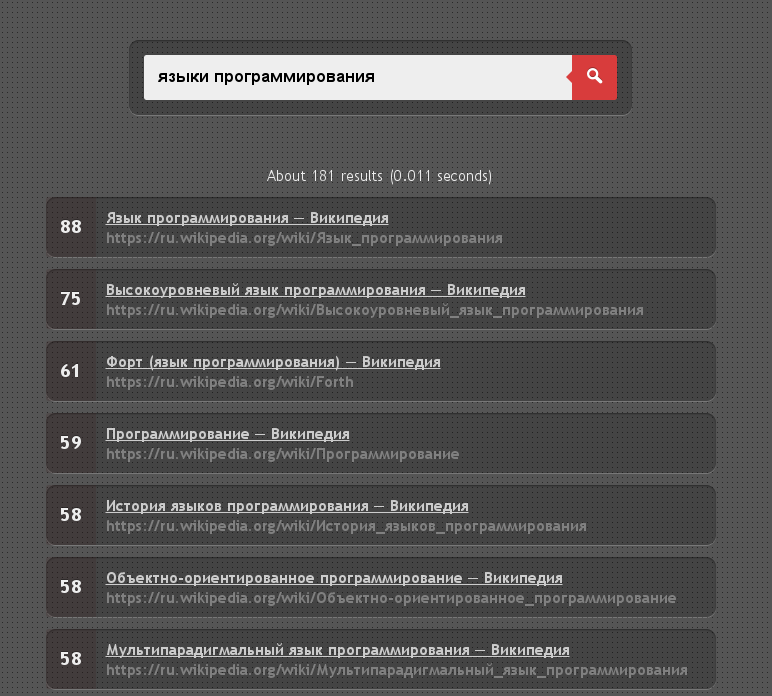
\includegraphics[width=.7\textwidth]{webpage-top.png}
  \caption{Поисковая страница.}
  \label{fig:webpage-top}
\end{figure}

\begin{figure}[h]
  \centering
  
\includegraphics[width=.7\textwidth]{webpage-bottom.png}
  \caption{Переключение групп страниц выдачи.}
  \label{fig:webpage-bottom}
\end{figure}

Все поисковые запросы со страницы выполняются без перезагрузки самой страницы.


\subsection*{Интерфейс командной строки}
Управление большей частью системы осуществляется через интерфейс командной строки. Входная точка представлена на листинге \ref{lst:cli-h}.
\begin{lstlisting}[caption=Интерфейс командной строки., label=lst:cli-h]
Usage: cli <command> ... (see -h)

Commands:
  crawl     browse WWW and index information
  pagerank  precalculate pagerank
  search    request for indexed information
  server    start the web server

Options:
  -d, --database  specify path to database           [string] [default: "se.db"]
  -h, --help      show help                                            [boolean]
\end{lstlisting}


\subsubsection*{Поисковой робот}
Данная команда запускает поискового робота, осуществляющего сбор и индексацию информации с сайтов сети (листинг \ref{lst:cli-crawl-h}). Процесс работы робота показан на листинге \ref{lst:cli-crawl}.
\begin{lstlisting}[caption=Интерфейс командной строки: поисковой робот., label=lst:cli-crawl-h]
Usage: cli crawl [options] <urls...>

Options:
  -d, --database         specify path to database    [string] [default: "se.db"]
  -h, --help             show help                                     [boolean]
  -m, --max-depth        how far the crawler can go        [number] [default: 4]
  -t, --timeout          a waiting time for a response    [number] [default: 15]
  -s, --max-size         max file size to process         [number] [default: 16]
  -r, --relax-time       how long to hold an empty domain [number] [default: 10]
  -g, --no-guessing      don't guess link relevant by url              [boolean]
  -i, --ignore-nofollow  ignore rel="nofollow"                         [boolean]
  -l, --link-stem-limit  limit stems per link             [number] [default: 10]
\end{lstlisting}

\begin{lstlisting}[caption=Интерфейс командной строки: поисковой робот., label=lst:cli-crawl]
D: 78523   I: 77890 (51210/h)   S: 1:32   Q: 4960|32329
[D] http://www.nature.com/nature/journal/v454/n7204/full/nature07130.html
~~~~~~~~~~~~~~~~~~~~~~~~~~~~~~~~~~~~~~~~~~~~~~~~~~~~~~~~~~~~~~~~~~~~~~~~~~~~~~
Downloaded: 78523
Indexed: 77890
Spent: 1:32
\end{lstlisting}


\subsubsection*{Постобработка}
Данная команда предназначена для запуска процесса постобработки~--- вычисления PageRank проиндексированных страниц и некоторой статистики (листинги \ref{lst:cli-pagerank-h} и \ref{lst:cli-pagerank}).
\begin{lstlisting}[caption=Интерфейс командной строки: постобработка., label=lst:cli-pagerank-h]
Usage: cli pagerank [options]

Options:
  -d, --database    specify path to database         [string] [default: "se.db"]
  -h, --help        show help                                          [boolean]
  -i, --iterations  the number of iterations              [number] [default: 30]
\end{lstlisting}

\begin{lstlisting}[caption=Интерфейс командной строки: постобработка., label=lst:cli-pagerank]
collecting inbound links
collecting initial data
iteration #0
iteration #1
...
iteration #28
iteration #29
filling index
updating info
analyzing tables
done
~~~~~~~~~~~~~~~~~~~~~~~~~~~~~~~~~~~~~~~~~~~~~~~~~~~~~~~~~~~~~~~~~~~~~~~~~~~~~~
Spent: 37m 53s
\end{lstlisting}


\subsubsection*{Сервер}
Данная команда запускает сервер, задачей которого является передача поисковой страницы пользователю с последующими принятием и обработкой поисковых запросов (листинги \ref{lst:cli-server-h} и \ref{lst:cli-server}).
\begin{lstlisting}[caption=Интерфейс командной строки: сервер., label=lst:cli-server-h]
Usage: cli server [options]

Options:
  -d, --database  specify path to database           [string] [default: "se.db"]
  -h, --help      show help                                            [boolean]
  -p, --port      specify the port                      [number] [default: 3000]
  -l, --limit     pages per request limit                 [number] [default: 15]
\end{lstlisting}

\begin{lstlisting}[caption=Интерфейс командной строки: сервер., label=lst:cli-server]
GET / - 7ms
GET /style.css - 2ms
GET /index.js - 1ms
GET /favicon.ico - 1ms
GET /search?q=python%20%D1%8F%D0%B7%D1%8B%D0%BA&o=0 - 23ms
\end{lstlisting}


\subsubsection*{Поиск}
Данная команда предназначена для проведения поиска и обладает большими возможностями по сравнению с поисковой страницей (листинги \ref{lst:cli-search-h} и \ref{lst:cli-search}).
\begin{lstlisting}[caption=Интерфейс командной строки: поиск., label=lst:cli-search-h]
Usage: cli search [options] <query>

Options:
  -d, --database  specify path to database           [string] [default: "se.db"]
  -h, --help      show help                                            [boolean]
  -l, --limit     the number of pages                     [number] [default: 10]
  -o, --offset    the number of skip pages                 [number] [default: 0]
  -v, --verbose   provide more useful info                               [count]
\end{lstlisting}

\begin{lstlisting}[caption=Интерфейс командной строки: поиск., label=lst:cli-search]
[77] Python (programming language) - Wikipedia, the free encyclopedia | htt...
[71] The Python Standard Library | http://docs.python.org/library/index.html
[69] Python-Dev Info Page | https://mail.python.org/mailman/listinfo/python...
[69] Sphinx 1.4.3 : Python Package Index | https://pypi.python.org/pypi/Sphinx
[69] PyPI - the Python Package Index | https://pypi.python.org/pypi
[66] Languages - Python Wiki | http://wiki.python.org/moin/Languages
[65] The Julia Language | http://julialang.org/
[62] The Python Tutorial — Python 3.5.1 documentation | http://docs.python....
[60] Python Developer’s Guide — Python Developer's Guide | https://docs.pyt...
[60] BeginnersGuide - Python Wiki | https://wiki.python.org/moin/BeginnersG...
~~~~~~~~~~~~~~~~~~~~~~~~~~~~~~~~~~~~~~~~~~~~~~~~~~~~~~~~~~~~~~~~~~~~~~~~~~~~~~
About 1208 results (0.036 seconds)
\end{lstlisting}

Данный команда позволяет контролировать детальность вывода аргументами \verb|-v| и \verb|-vv| (листинг \ref{lst:cli-search-vv}).
\begin{lstlisting}[caption=Интерфейс командной строки: поиск., label=lst:cli-search-vv]
[88] Язык программирования — Википедия | https://ru.wikipedia.org/wiki/Язык...
     scores: wbm=0.91 hbm=0.99 cnt=0.64 pos=1.00 ref=1.00 pr=0.49
     words: 2402   heads: 11   total pos: 3   PR: 1.01   ref PR: 40.29

[75] Высокоуровневый язык программирования — Википедия | https://ru.wikiped...
     scores: wbm=0.90 hbm=1.00 cnt=0.12 pos=1.00 ref=0.91 pr=0.10
     words: 469   heads: 4   total pos: 5   PR: 0.33   ref PR: 11.86

[59] Программирование — Википедия | https://ru.wikipedia.org/wiki/Программи...
     scores: wbm=0.91 hbm=0.62 cnt=0.16 pos=0.94 ref=0.52 pr=0.29
     words: 628   heads: 2   total pos: 81   PR: 0.67   ref PR: 6.90

[58] История языков программирования — Википедия | https://ru.wikipedia.org...
     scores: wbm=0.86 hbm=1.00 cnt=0.25 pos=1.00 ref=0.02 pr=0.01
     words: 948   heads: 4   total pos: 5   PR: 0.17   ref PR: 0.35

[58] Объектно-ориентированное программирование — Википедия | https://ru.wik...
     scores: wbm=0.78 hbm=0.52 cnt=1.00 pos=0.91 ref=0.16 pr=0.24
     words: 3794   heads: 4   total pos: 121   PR: 0.58   ref PR: 2.25
  ...
~~~~~~~~~~~~~~~~~~~~~~~~~~~~~~~~~~~~~~~~~~~~~~~~~~~~~~~~~~~~~~~~~~~~~~~~~~~~~~
  About 181 results (0.025 seconds)
\end{lstlisting}
